\section{Fundamentação matemática}\label{cap:matematica}
% orçamento: 1.500 palavras

O capítulo anterior terminou com dois problemas que a física sozinha não resolve: escrever uma órbita como soma de movimentos circulares e integrar numericamente a \autoref{eq:nbody}. Este capítulo trata dos dois. A primeira metade vai das séries de Fourier aos epiciclos e chega à forma fechada dos coeficientes de uma órbita kepleriana. A segunda metade trata dos integradores numéricos e da aritmética de computador.

\subsection{Séries de Fourier}\label{sec:fourier-real}

\begin{paracomecar}
Uma série de Fourier escreve uma curva que se repete como soma de ondas simples, cada uma com uma frequência inteira: uma volta por período, duas voltas, três voltas, e assim por diante. Quanto mais ondas se somam, mais fiel fica a cópia.
\end{paracomecar}

Seja $f$ uma função real periódica de período $T$, com frequência angular $\omega = 2\pi/T$. Sob condições bem gerais, que incluem todas as órbitas fechadas deste trabalho, vale \cite{thomas2009}
\begin{equation}
  f(t) = \frac{a_0}{2} + \sum_{n=1}^{\infty}\bigl[a_n\cos(n\omega t) + b_n\sin(n\omega t)\bigr],
  \label{eq:fourier-real}
\end{equation}
com coeficientes
\begin{equation}
  a_n = \frac{2}{T}\int_0^T f(t)\cos(n\omega t)\,\dd t,\qquad
  b_n = \frac{2}{T}\int_0^T f(t)\sin(n\omega t)\,\dd t.
  \label{eq:fourier-coef-real}
\end{equation}
Essas são as equações 2 a 5 de \citeonline{farias2016}. Para uma curva no plano, $(x(t),y(t))$, aplica-se a \autoref{eq:fourier-real} a cada coordenada, obtendo quatro famílias de coeficientes, $a_n,b_n$ para $x$ e $c_n,d_n$ para $y$.

\subsection{A forma complexa e os epiciclos}\label{sec:fourier-complexa}

Escreva a posição no plano como um número complexo, $z(t) = x(t) + \ii\,y(t)$. Pela fórmula de Euler, $e^{\ii\theta} = \cos\theta + \ii\sin\theta$ é um ponto do círculo unitário no ângulo $\theta$, e $e^{\ii n\omega t}$ é um ponto que gira sobre esse círculo com velocidade angular constante $n\omega$. Usando o período como unidade de tempo ($T=1$, $t\in[0,1)$), a série de Fourier complexa de $z$ é
\begin{equation}
  z(t) = \sum_{n=-\infty}^{\infty} c_n\,e^{2\pi\ii n t},
  \qquad
  c_n = \int_0^1 z(t)\,e^{-2\pi\ii n t}\,\dd t.
  \label{eq:fourier-complexa}
\end{equation}
A fórmula dos coeficientes vem da \emph{ortogonalidade} das exponenciais: $\int_0^1 e^{2\pi\ii (m-n)t}\dd t$ vale 1 se $m=n$ e 0 caso contrário. Multiplicando a série por $e^{-2\pi\ii n t}$ e integrando, todos os termos se anulam menos o de índice $n$.

\begin{proposicao}[cada termo é um epiciclo]\label{prop:epiciclo}
O termo $c_n e^{2\pi\ii nt}$, com $c_n = |c_n|e^{\ii\varphi_n}$, é um ponto que percorre um círculo de raio $|c_n|$ com velocidade angular constante $2\pi n$ e fase inicial $\varphi_n$. Para $n>0$ o giro é anti-horário, isto é, no mesmo sentido da órbita; para $n<0$ é horário; para $n=0$ o termo não gira e é um deslocamento fixo.
\end{proposicao}

\begin{proof}
$c_n e^{2\pi\ii nt} = |c_n|\,e^{\ii(2\pi n t + \varphi_n)}$, cujo módulo é constante e igual a $|c_n|$ e cujo argumento cresce linearmente com taxa $2\pi n$.
\end{proof}

A soma da \autoref{eq:fourier-complexa} é, portanto, uma \emph{cadeia de epiciclos}. Partindo do ponto fixo $c_0$, monta-se o círculo de raio $|c_{n_1}|$; na ponta do seu raio, o círculo de raio $|c_{n_2}|$; e assim por diante. A ponta do último elo é exatamente a soma da série truncada, e não uma ilustração ao lado dela (\autoref{fig:epiciclos}). O termo de raio maior, $n=1$, é o \emph{deferente}, e o termo fixo $c_0$ faz o papel do \emph{excêntrico}, o deslocamento entre o centro do deferente e o Sol.

\begin{figure}[htb]
  \centering
  \caption{Cadeia de epiciclos de uma órbita kepleriana com $e = 0{,}5$}
  \label{fig:epiciclos}
  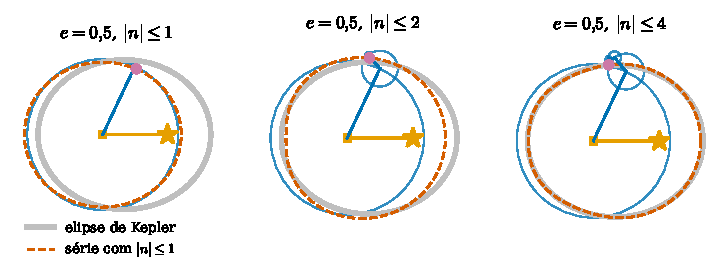
\includegraphics[width=\textwidth]{epiciclos.pdf}
  \legend{Em cinza, a elipse; tracejado, a série truncada em $|n|\leq N$. O segmento amarelo vai do Sol (estrela) ao termo fixo $c_0$; os círculos azuis são os epiciclos, montados em ordem decrescente de raio, e o ponto rosa é a ponta da cadeia no instante $t = 0{,}18\,T$. A excentricidade foi exagerada para tornar visíveis os epiciclos menores. Fonte: elaborada pelos autores.}
\end{figure}

\subsubsection{Da forma real para a complexa}

As duas formas carregam a mesma informação. Substituindo $\cos\theta = (e^{\ii\theta}+e^{-\ii\theta})/2$ e $\sin\theta = (e^{\ii\theta}-e^{-\ii\theta})/(2\ii)$ em $z = x + \ii y$, com $x$ e $y$ na forma \eqref{eq:fourier-real}, obtém-se para $n\geq1$
\begin{equation}
  c_{n} = \frac{(a_n + d_n) + \ii\,(c_n^{(y)} - b_n)}{2},
  \qquad
  c_{-n} = \frac{(a_n - d_n) + \ii\,(c_n^{(y)} + b_n)}{2},
  \label{eq:real-complexa}
\end{equation}
em que escrevemos $c_n^{(y)}$ para o coeficiente de cosseno de $y$, para não confundir com o coeficiente complexo. Os módulos
\[
  |c_n| = \tfrac12\sqrt{(a_n+d_n)^2 + (c_n^{(y)}-b_n)^2},\qquad
  |c_{-n}| = \tfrac12\sqrt{(a_n-d_n)^2 + (c_n^{(y)}+b_n)^2}
\]
são exatamente os raios $R_n$ e $r_n$ das equações 22 e 23 de \citeonline{farias2016}, que o TCC chamou de epiciclo de frequência $n\omega$ e epiciclo que gira em sentido contrário.

\begin{licao}[: senos e cossenos separados não são epiciclos]
As versões 1 e 2 do programa decompunham $x$ e $y$ separadamente, como na \autoref{eq:fourier-real}. Isso reconstrói a curva corretamente, mas um par $a_n\cos + b_n\sin$ em $x$ junto com $c_n\cos + d_n\sin$ em $y$ é uma \emph{elipse} alinhada aos eixos, e não um círculo. Para desenhar a cadeia histórica de epiciclos, a versão 3D passou a usar a série complexa, com $n$ percorrendo também os inteiros negativos. O TCC já fazia essa combinação ao calcular $R_n$ e $r_n$; o código levou duas versões para chegar lá.
\end{licao}

\subsection{A órbita de Kepler como função do tempo}\label{sec:param-tempo}

Para aplicar a \autoref{eq:fourier-complexa} a uma órbita é preciso escolher o parâmetro $t$. Há duas escolhas naturais, e elas \emph{não} são equivalentes:

\begin{itemize}
  \item \textbf{no tempo}: $z(t)$ é a posição do planeta no instante $t$. Pela segunda lei de Kepler, pontos igualmente espaçados no tempo ficam juntos perto do afélio, onde o planeta anda devagar, e espalhados perto do periélio (\autoref{fig:amostragem}a);
  \item \textbf{no ângulo}: $z(\theta) = r(\theta)e^{\ii\theta}$ é o ponto da elipse na direção $\theta$ vista do Sol, sem relação com o tempo (\autoref{fig:amostragem}b).
\end{itemize}

\begin{figure}[htb]
  \centering
  \caption{Trinta e seis pontos de uma mesma elipse ($e=0{,}5$) escolhidos de dois modos}
  \label{fig:amostragem}
  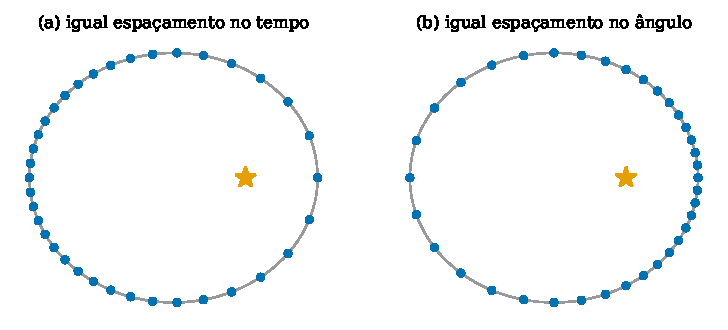
\includegraphics[width=0.85\textwidth]{amostragem.pdf}
  \legend{Em (a), cada ponto está a $T/36$ do seguinte, e o espaçamento desigual é a segunda lei de Kepler. Em (b), cada ponto está a $10^\circ$ do seguinte, visto do Sol (estrela). Fonte: elaborada pelos autores.}
\end{figure}

As duas são funções periódicas diferentes da mesma curva, com coeficientes diferentes. Só a parametrização no tempo tem significado físico: nela, ``girar com velocidade angular constante'' descreve o que um epiciclo faz \emph{no céu}, e é nela que o modelo de Copérnico pode ser comparado. A primeira versão do projeto amostrava em ângulo, e a \autoref{fig:angulo-tempo} mostra o efeito: para $e = 0{,}5$, o termo fixo vale $c_0 = -0{,}232\,a$ na amostragem em ângulo e $c_0 = -0{,}750\,a$ no tempo.

\begin{figure}[htb]
  \centering
  \caption{O mesmo cálculo de Fourier em duas parametrizações}
  \label{fig:angulo-tempo}
  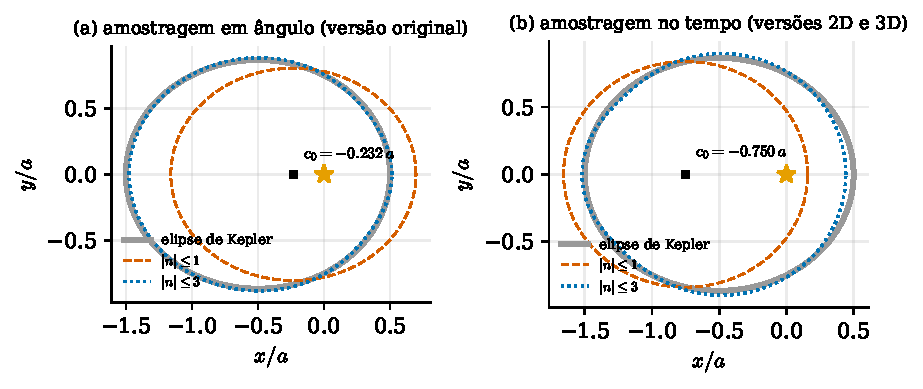
\includegraphics[width=0.95\textwidth]{angulo_tempo.pdf}
  \legend{Órbita hipotética com $e=0{,}5$. O quadrado preto marca $c_0$. As reconstruções com $|n|\leq1$ diferem: são aproximações de funções diferentes. Fonte: elaborada pelos autores.}
\end{figure}

\subsection{Os coeficientes em forma fechada}\label{sec:bessel}

Para a órbita kepleriana parametrizada no tempo, os coeficientes de Fourier têm forma fechada, escrita em termos das funções que Bessel estudou sistematicamente no início do século XIX, justamente no contexto do problema de Kepler \cite{watson1944,colwell1993}. Use a anomalia média $M = 2\pi t$ como variável e o periélio sobre o eixo real. Pela \autoref{eq:perifocal}, $z = a(\cos E - e) + \ii b\sin E$.

\subsubsection{O termo fixo}

Pela equação de Kepler, $\dd M = (1 - e\cos E)\,\dd E$. Então
\begin{align}
  c_0 = \frac{1}{2\pi}\int_0^{2\pi} z\,\dd M
  &= \frac{1}{2\pi}\int_0^{2\pi}\bigl[a(\cos E - e) + \ii b\sin E\bigr](1-e\cos E)\,\dd E \nonumber\\
  &= \frac{a}{2\pi}\int_0^{2\pi}\bigl(\cos E - e - e\cos^2E + e^2\cos E\bigr)\dd E \;+\; 0
   = a\Bigl(-e - \frac{e}{2}\Bigr),
\end{align}
porque $\cos E$ e $\sin E\cos E$ têm média nula e $\cos^2E$ tem média $\tfrac12$. Logo
\begin{equation}
  \boxed{\;c_0 = -\tfrac{3}{2}\,a e\;}
  \label{eq:c0}
\end{equation}
A posição média do planeta \emph{no tempo} fica a $\tfrac32 ae$ do Sol, do lado do afélio, e não a $ae$, que é onde está o centro geométrico da elipse. A diferença é a segunda lei: o planeta passa mais tempo longe do Sol, e a média temporal se desloca para lá.

\subsubsection{Os demais termos}

Para $n\neq0$, integra-se por partes e troca-se a variável para $E$; os detalhes estão no \autoref{ap:derivacoes}. Usando a representação integral de Bessel, $J_k(x) = \frac{1}{2\pi}\int_0^{2\pi}\cos(k\tau - x\sin\tau)\,\dd\tau$, chega-se a
\begin{equation}
  \boxed{\;c_n = \frac{a}{n}\,J_n'(ne) + \frac{b}{ne}\,J_n(ne),\qquad n\neq 0,\;}
  \label{eq:cn-bessel}
\end{equation}
válida para $n$ positivo e negativo, com $b = a\sqrt{1-e^2}$. Os coeficientes são todos reais: com o periélio no eixo real, a órbita é simétrica em relação a esse eixo. O \autoref{cap:resultados} confere a \autoref{eq:cn-bessel} contra os coeficientes calculados numericamente pelo programa; a diferença fica na casa de $10^{-16}$\,UA, o arredondamento da máquina.

\subsubsection{Desenvolvimento em pequena excentricidade}\label{sec:pequeno-e}

Para argumentos pequenos, $J_n(x)\approx (x/2)^n/n!$. Expandindo a \autoref{eq:cn-bessel} nas primeiras potências de $e$:
\begin{equation}
  c_0 = -\tfrac32 ae,\quad
  c_1 = a\Bigl(1-\tfrac{e^2}{2}\Bigr) + O(e^4),\quad
  c_2 = \tfrac12 ae + O(e^3),\quad
  c_{-1} = \tfrac18 ae^2 + O(e^4),
  \label{eq:pequeno-e}
\end{equation}
e todos os demais são de ordem $e^2$ ou superior. Portanto, até primeira ordem em $e$,
\begin{equation}
  \boxed{\;z(M) \;\approx\; -\tfrac32 ae \;+\; a\,e^{\ii M} \;+\; \tfrac12 ae\,e^{2\ii M}\;}
  \label{eq:copernico-fourier}
\end{equation}
A órbita de Kepler, vista como série de Fourier no tempo, é \emph{um deslocamento fixo, um deferente e um epiciclo que gira com o dobro da frequência}, com raios na razão $\tfrac32 : 1 : \tfrac12$ vezes $a$, $a$ e $ae$. O \autoref{sec:copernico-revisitado} mostra que essa é, termo a termo, a construção de Copérnico.

\subsection{Discretização: a série de Fourier no computador}\label{sec:dft}

No programa, a órbita entra como $A$ amostras igualmente espaçadas no tempo, $z_k = z(k/A)$, $k=0,\dots,A-1$, e a integral da \autoref{eq:fourier-complexa} vira a soma
\begin{equation}
  \hat c_n = \frac{1}{A}\sum_{k=0}^{A-1} z_k\,e^{-2\pi\ii nk/A},
  \label{eq:dft}
\end{equation}
a transformada discreta de Fourier (DFT) \cite{press2007}. A soma reproduz a integral exatamente para funções com espectro limitado, mas em geral cada coeficiente calculado é a soma de todos os coeficientes verdadeiros que coincidem com ele nas amostras: $\hat c_n = \sum_{m} c_{n+mA}$. Esse é o fenômeno de \emph{aliasing}. Ele impõe duas regras ao programa:

\begin{enumerate}
  \item com $A$ amostras, só os harmônicos com $|n| < A/2$ são recuperáveis (critério de Nyquist). O programa usa $A = 720$ e $|n|\leq 24$ e \emph{recusa}, com erro explícito, qualquer combinação que viole $2N < A$, em vez de devolver um número errado;
  \item mesmo dentro do limite, o erro depende de quão depressa $|c_n|$ decai. Para órbitas muito alongadas o espectro decai devagar, e a dobra dos termos altos contamina os baixos. Medido no programa, com 720 amostras: erro de coeficiente de $3\times10^{-16}$\,UA em $e = 0{,}6$, $10^{-14}$ em $e = 0{,}9$ e $10^{-8}$ em $e = 0{,}95$.
\end{enumerate}

O desvio da série truncada é medido ponto a ponto contra as próprias amostras. Pela identidade de Parseval, o desvio quadrático médio da série truncada em $|n|\leq N$ é $\bigl(\sum_{|n|>N}|c_n|^2\bigr)^{1/2}$: cada termo omitido contribui com o quadrado do próprio raio. É por isso que a convergência é tão rápida para órbitas quase circulares, em que os raios dos epiciclos caem como potências de $e$.

\subsection{Integração numérica}\label{sec:integradores}

\begin{paracomecar}
O computador não resolve a equação do movimento de uma vez. Ele dá passos: sabendo onde cada planeta está e com que velocidade, calcula onde estará meio dia depois, e repete. O problema é que os pequenos erros de cada passo se somam e, com o tempo, deformam a órbita.
\end{paracomecar}

\subsubsection{O problema de um método ingênuo}

O método mais simples, o de Euler, atualiza posição e velocidade usando os valores do início do passo: $\vr_{k+1} = \vr_k + \Delta t\,\vv_k$, $\vv_{k+1} = \vv_k + \Delta t\,\va(\vr_k)$. Para uma órbita circular, cada passo leva o corpo pela tangente, ligeiramente para fora do círculo, e a energia cresce a cada volta. Depois de algumas centenas de órbitas, o planeta escapa. Métodos de ordem mais alta, como o Runge--Kutta clássico de quarta ordem (RK4), erram muito menos em cada passo, mas o erro de energia continua tendo sinal sistemático e cresce sem limite, só que mais devagar.

\subsubsection{Integradores simpléticos}

As equações de Newton para a gravitação têm estrutura hamiltoniana: o estado é um ponto no espaço de fase $(\vr,\vv)$ e a evolução exata preserva volumes nesse espaço (teorema de Liouville). Um integrador \emph{simplético} é um método cujo passo também preserva essa estrutura \cite{hairer2006}. A consequência prática, demonstrada pela análise de erro regressiva, é que a solução numérica de um integrador simplético é a solução \emph{exata} de um hamiltoniano ligeiramente modificado, $\tilde H = H + O(\Delta t^p)$. Como $\tilde H$ se conserva exatamente, a energia verdadeira $H$ apenas oscila em torno do valor inicial, com amplitude $O(\Delta t^p)$, sem crescimento secular, por tempos exponencialmente longos.

\subsubsection{Leapfrog (Verlet)}

O integrador simplético mais simples é o \emph{leapfrog}, ou Verlet de velocidade \cite{verlet1967}. Ele alterna meio impulso, um deslocamento inteiro e outro meio impulso:
\begin{align}
  \vv_{k+1/2} &= \vv_k + \tfrac12\Delta t\,\va(\vr_k), \nonumber\\
  \vr_{k+1}   &= \vr_k + \Delta t\,\vv_{k+1/2}, \label{eq:leapfrog}\\
  \vv_{k+1}   &= \vv_{k+1/2} + \tfrac12\Delta t\,\va(\vr_{k+1}). \nonumber
\end{align}
É de segunda ordem, simétrico no tempo (dar um passo com $-\Delta t$ desfaz exatamente o passo com $+\Delta t$, a menos do arredondamento) e custa uma avaliação de força por passo, porque $\va(\vr_{k+1})$ é reaproveitada no passo seguinte. Denote por $S_2(\Delta t)$ esse passo.

\subsubsection{A composição de Yoshida}

\citeonline{yoshida1990} mostrou como construir métodos simpléticos de ordem mais alta compondo passos de um método simétrico de ordem 2. A versão de quarta ordem é
\begin{equation}
  S_4(\Delta t) = S_2(w_1\Delta t)\;S_2(w_0\Delta t)\;S_2(w_1\Delta t).
  \label{eq:yoshida}
\end{equation}
Os pesos saem de duas condições. A soma dos subpassos precisa dar o passo inteiro, $2w_1 + w_0 = 1$. E o termo de erro de terceira ordem, que em cada $S_2(h)$ é proporcional a $h^3$, precisa se cancelar: $2w_1^3 + w_0^3 = 0$. Resolvendo,
\begin{equation}
  w_1 = \frac{1}{2 - 2^{1/3}} \approx 1{,}35120719,\qquad
  w_0 = -\frac{2^{1/3}}{2 - 2^{1/3}} \approx -1{,}70241438.
  \label{eq:pesos-yoshida}
\end{equation}
O peso central é \emph{negativo}: o subpasso do meio anda para trás no tempo. O método resultante é simplético, simétrico, de quarta ordem e custa três avaliações de força por passo.

\begin{paraaprofundar}[: por que os pesos são escritos como números e não calculados]
O programa grava $w_1$ e $w_0$ como literais de 17 algarismos em vez de calcular $1/(2-\sqrt[3]{2})$ em tempo de execução. A razão é a reprodutibilidade: assim o valor não depende de a função de raiz cúbica de cada motor de JavaScript concordar com as demais no último bit. Um teste automatizado confere os literais contra a fórmula com tolerância de uma unidade na última casa.
\end{paraaprofundar}

\subsubsection{Passo fixo}

O simulador usa $S_4$ com passo \emph{fixo} de $\Delta t = 0{,}5$ dia, por duas razões independentes. Passo variável destrói a propriedade simplética, a menos de técnicas especiais. E com passo fixo a data exibida na tela é sempre exatamente $t_0 + k\cdot 0{,}5$ dia, sem arredondamento acumulado. O valor de meio dia foi escolhido por medição (\autoref{sec:res-integradores}).

\subsubsection{Interpolação para o desenho}

A física anda de meio em meio dia, mas a tela é redesenhada 60 ou 120 vezes por segundo. A 1 dia por segundo, isso daria dois saltos visíveis por segundo. O programa desenha uma posição intermediária entre dois estados integrados consecutivos usando a \emph{interpolação cúbica de Hermite}, que usa posição e velocidade nas duas pontas:
\begin{equation}
  \vr(\alpha) = h_{00}(\alpha)\,\vr_k + h_{10}(\alpha)\,\Delta t\,\vv_k + h_{01}(\alpha)\,\vr_{k+1} + h_{11}(\alpha)\,\Delta t\,\vv_{k+1},
  \qquad 0\le\alpha\le1,
  \label{eq:hermite}
\end{equation}
com $h_{00} = 2\alpha^3 - 3\alpha^2 + 1$, $h_{10} = \alpha^3 - 2\alpha^2 + \alpha$, $h_{01} = -2\alpha^3 + 3\alpha^2$ e $h_{11} = \alpha^3 - \alpha^2$. A curva resultante é contínua em posição e em velocidade nas fronteiras dos passos. Uma alternativa mais barata, extrapolar por Taylor a partir do estado atual, foi descartada por medição: em meio passo o termo de terceira ordem vale 213\,km em Mercúrio, 4\,\% do diâmetro do planeta, e isso aparecia como um tranco na fronteira de cada passo. A data escrita na tela é a do instante interpolado, $t_k + \alpha\Delta t$, de modo que o número na tela sempre corresponde ao desenho.

\subsection{Aritmética de ponto flutuante}\label{sec:float}

Computadores representam números reais com um número finito de algarismos binários, no padrão IEEE 754 \cite{ieee754,goldberg1991}. Em precisão dupla (\emph{float64}) há cerca de 16 algarismos decimais significativos; em precisão simples (\emph{float32}), cerca de 7. Toda a física do simulador roda em float64, e nessa precisão a posição de Netuno, a 30\,UA, fica quantizada em cerca de $10^{-15}\times 30\UA \approx 1\,\mathrm{mm}$.

As placas gráficas, porém, trabalham em float32, que em 30\,UA quantiza a centenas de quilômetros. O problema não é o valor em si, que seria invisível na tela, mas a \emph{subtração de dois números grandes e próximos}. A câmera a 30\,UA da origem olhando um planeta também a 30\,UA precisa calcular a diferença entre as duas posições, e em float32 essa diferença perde quase todos os algarismos significativos. A cena treme. A solução, descrita na \autoref{sec:origem-flutuante}, é fazer essa subtração em float64, na CPU, antes de enviar qualquer coisa para a placa.

\subsection{Escala de desenho}\label{sec:compressao}

Netuno está 77 vezes mais longe do Sol que Mercúrio. Numa tela que mostra o sistema inteiro em escala real, os quatro planetas internos ocupam uma área do tamanho de um dedo. O programa oferece, como opção desligada por padrão, o \emph{modo maquete}, que comprime as distâncias desenhadas por
\begin{equation}
  r_\text{desenho} = R\,\sqrt{r/R},\qquad R = 1\UA,
  \label{eq:compressao}
\end{equation}
preservando direções e mantendo a órbita da Terra inalterada (\autoref{fig:compressao}). A raiz foi preferida ao logaritmo porque é monótona, suave e vale zero em zero, enquanto o logaritmo leva o centro a $-\infty$ e exige um piso arbitrário. A razão entre o planeta mais distante e o mais próximo cai de 77:1 para 8,8:1.

\begin{figure}[htb]
  \centering
  \caption{A compressão de distâncias do modo maquete}
  \label{fig:compressao}
  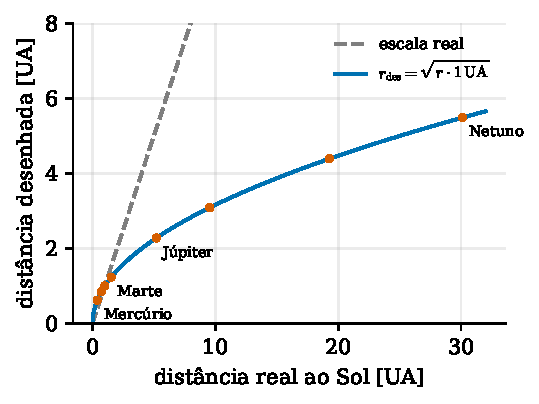
\includegraphics[width=0.62\textwidth]{compressao.pdf}
  \legend{Os pontos marcam os semieixos dos oito planetas. Fonte: elaborada pelos autores.}
\end{figure}

A compressão altera só a coordenada de desenho, nunca o estado físico. A iluminação continua usando a distância real, para que Netuno, desenhado a 5,5\,UA do Sol, não receba trinta vezes mais luz do que recebe. Com a compressão ligada, a tela avisa por escrito.
